% Created 2017-06-20 Tue 00:49
% Intended LaTeX compiler: pdflatex
\documentclass[11pt]{article}
\usepackage[utf8]{inputenc}
\usepackage[T1]{fontenc}
\usepackage{graphicx}
\usepackage{grffile}
\usepackage{longtable}
\usepackage{wrapfig}
\usepackage{rotating}
\usepackage[normalem]{ulem}
\usepackage{amsmath}
\usepackage{textcomp}
\usepackage{amssymb}
\usepackage{capt-of}
\usepackage{hyperref}
\usepackage{xfrac}
\let\originalleft\left
\let\originalright\right
\renewcommand{\left}{\mathopen{}\mathclose\bgroup\originalleft}
\renewcommand{\right}{\aftergroup\egroup\originalright}
\author{Kevin Orr}
\date{\today}
\title{Project 1 Analysis}
\hypersetup{
 pdfauthor={Kevin Orr},
 pdftitle={Project 1 Analysis},
 pdfkeywords={},
 pdfsubject={},
 pdfcreator={Emacs 25.1.2 (Org mode 9.0.8)}, 
 pdflang={English}}
\begin{document}

\maketitle
\tableofcontents


\section{Results}
\label{sec:orgcc3118e}

The provided program was run with all combinations of the sorting algorithms selection sort,
insertion sort, merge sort, and quicksort; and input arrays that are strictly increasing, strictly
decreasing, constant, or randomized. From these results we derive four variables:
\(n_{min}, t_{min}, n_{max}, t_{max}\). They are defined as follows:

\begin{description}
\item[$n_{min}$] The smallest array that took at least 20 ms to sort
\item[$t_{min}$] The time it took to sort the array of size $n_{min}$
\item[$n_{max}$] The largest array that took no longer than 10 minutes to sort
\item[$t_{min}$] The time it took to sort the array of size $n_{max}$
\end{description}

\begin{center}
\begin{tabular}{llrrrr}
Algorithm & Input Type & \(n_{min}\) & \(t_{min}\) & \(n_{max}\) & \(t_{max}\)\\
\hline
selection & increasing & 10000 & 82 & 100000 & 8285\\
selection & decreasing & 10000 & 84 & 100000 & 8421\\
selection & constant & 10000 & 82 & 100000 & 8283\\
selection & random & 10000 & 84 & 100000 & 8420\\
\hline
insertion & increasing & 10000000 & 24 & 1000000000 & 2472\\
insertion & decreasing & 10000 & 46 & 1000000 & 463830\\
insertion & constant & 10000000 & 24 & 1000000000 & 2477\\
insertion & random & 10000 & 46 & 1000000 & 464006\\
\hline
mergesort & increasing & 1000000 & 42 & 1000000000 & 62201\\
mergesort & decreasing & 1000000 & 115 & 1000000000 & 172232\\
mergesort & constant & 1000000 & 43 & 1000000000 & 62500\\
mergesort & random & 1000000 & 115 & 1000000000 & 172469\\
\hline
quicksort & increasing & 1000000 & 33 & 1000000000 & 46599\\
quicksort & decreasing & 1000000 & 116 & 1000000000 & 170442\\
quicksort & constant & 10000 & 35 & 100000 & 3512\\
quicksort & random & 1000000 & 116 & 1000000000 & 170431\\
\end{tabular}
\end{center}

\section{Plots}
\label{sec:orgae00a53}

The following plots show the behavior for our four sorting algorithms. Each algorithm was
tested with array sizes of \(n 10^m \le 10^9\) for
\(n \in \{1, 2, 3, 4, 5, 6, 7, 8, 9\}, m \in \{0, 1, 2, 3, 4, 5, 6, 7, 8, 9\}\).

\subsection{Selection Sort}
\label{sec:orgc278a57}
\begin{center}
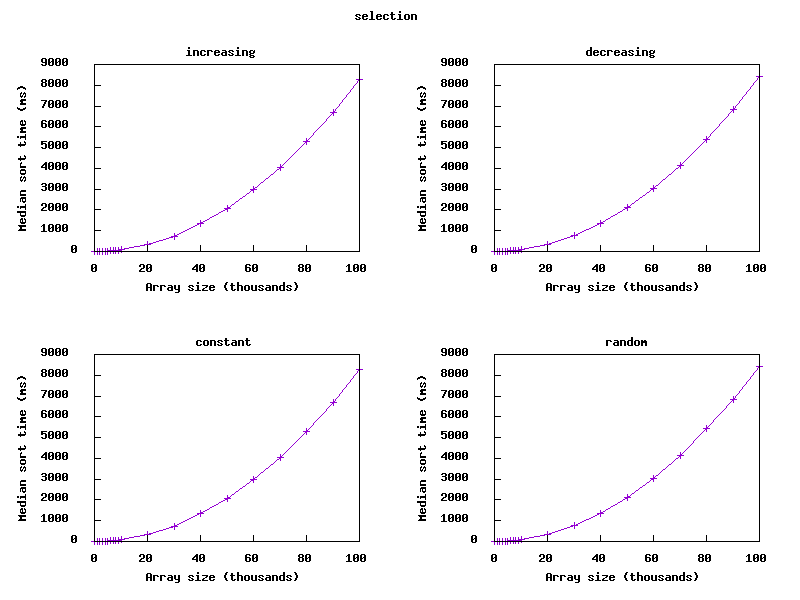
\includegraphics[width=10cm]{./output/selection.png}
\end{center}

\subsection{Insertion Sort}
\label{sec:orgec204bc}
\begin{center}
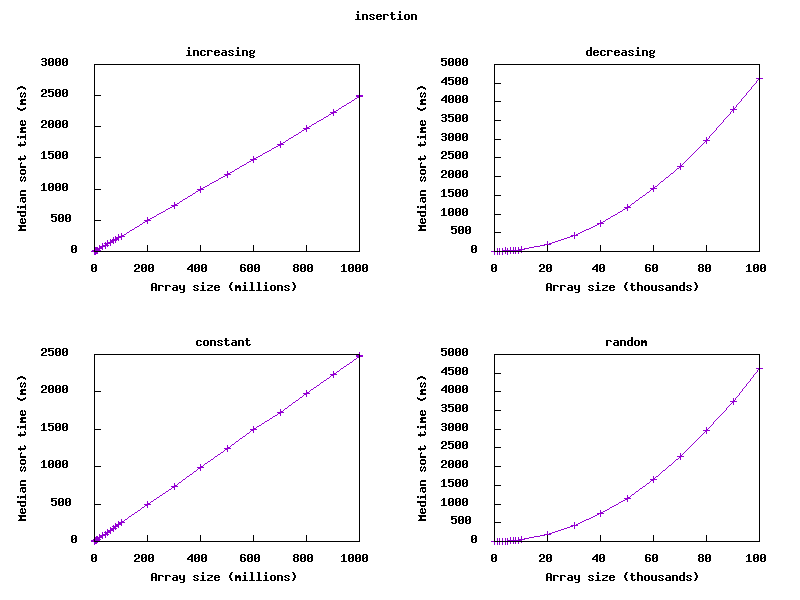
\includegraphics[width=10cm]{./output/insertion.png}
\end{center}

\subsection{Merge Sort}
\label{sec:org05d5c9a}
\begin{center}
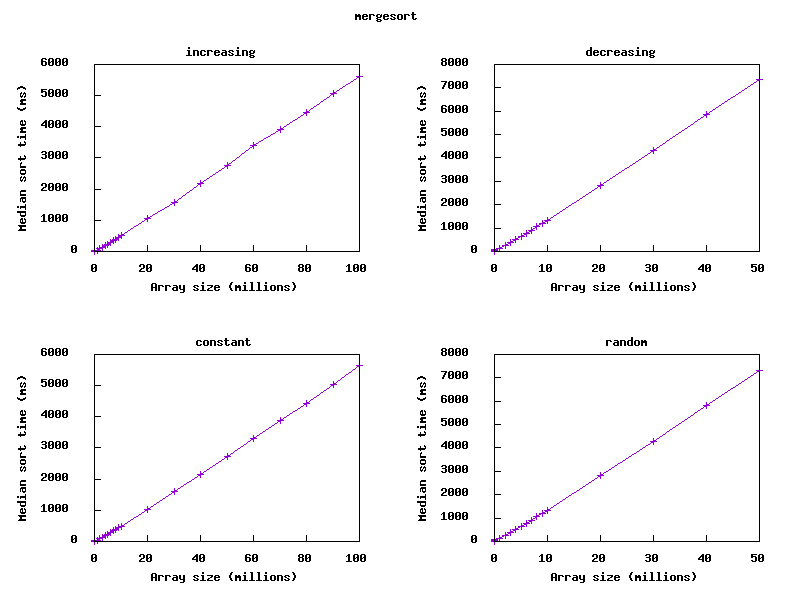
\includegraphics[width=10cm]{./output/mergesort.png}
\end{center}

\subsection{QuickSort}
\label{sec:orgff79b59}
\begin{center}
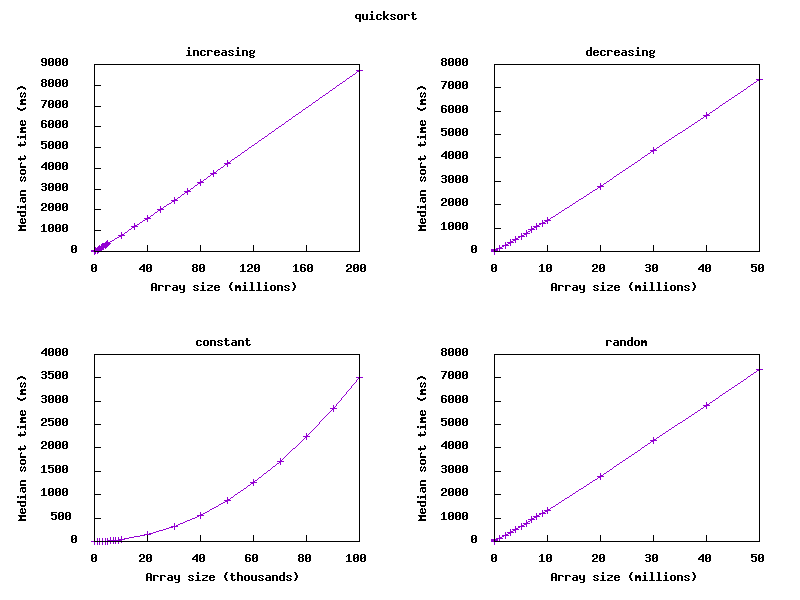
\includegraphics[width=10cm]{./output/quicksort.png}
\end{center}

\section{Analysis}
\label{sec:orgc7fdbd9}

The results from section \ref{sec:orgcc3118e} were then used in the following calculations to determine the
time complexity of the sorting algorithms. For each
\(f_i \in \left\{ f_1(n) = n, f_2(n) = n \lg n, f_3(n) = n^2 \right\}\),
I compared \(f_i(n_{max})/f_i(n_{min})\) to \(t_{max}/t_{min}\). Ideally, the first ratio should
be sufficiently close to the second when \(f_i(n)\) corresponds to the theoretical time complexity
of the algorithm of interest. These ratios are shown in the following table:

\begin{center}
\begin{tabular}{llrrrr}
Algorithm & Input Type & \(t_{max}/t_{min}\) & \(n_{max}/n_{min}\) & \(\frac{n_{max} \lg n_{max}}{n_{min} \lg n_{min}}\) & \(n_{max}^2/n_{min}^2\)\\
\hline
selection & increasing & 101.03658 & 10.0 & 12.5 & 100.0\\
selection & decreasing & 100.25 & 10.0 & 12.5 & 100.0\\
selection & constant & 101.01219 & 10.0 & 12.5 & 100.0\\
selection & random & 100.2381 & 10.0 & 12.5 & 100.0\\
\hline
insertion & increasing & 103.0 & 100.0 & 128.57143 & 10000.0\\
insertion & decreasing & 10083.261 & 100.0 & 150.0 & 10000.0\\
insertion & constant & 103.208336 & 100.0 & 128.57143 & 10000.0\\
insertion & random & 10087.087 & 100.0 & 150.0 & 10000.0\\
\hline
mergesort & increasing & 1480.9762 & 1000.0 & 1500.0 & 1000000.0\\
mergesort & decreasing & 1497.6696 & 1000.0 & 1500.0 & 1000000.0\\
mergesort & constant & 1453.4884 & 1000.0 & 1500.0 & 1000000.0\\
mergesort & random & 1499.7305 & 1000.0 & 1500.0 & 1000000.0\\
\hline
quicksort & increasing & 1412.091 & 1000.0 & 1500.0 & 1000000.0\\
quicksort & decreasing & 1469.3276 & 1000.0 & 1500.0 & 1000000.0\\
quicksort & constant & 100.34286 & 10.0 & 12.5 & 100.0\\
quicksort & random & 1469.2328 & 1000.0 & 1500.0 & 1000000.0\\
\end{tabular}
\end{center}

\subsection{Theoretical time complexities}
\label{sec:org9189fe7}

\begin{center}
\begin{tabular}{llll}
Algorithm & Best-case & Average-case & Worst-case\\
\hline
selection & \(\Theta\left(n^2\right)\) & \(\Theta\left(n^2\right)\) & \(\Theta\left(n^2\right)\)\\
insertion & \(\Omega(n)\) & \(\Theta\left(n^2\right)\) & \(\textrm{O}\left(n^2\right)\)\\
mergesort & \(\Theta(n \lg n)\) & \(\Theta(n \lg n)\) & \(\Theta(n \lg n)\)\\
quicksort & \(\Omega(n \lg n)\) & \(\Theta(n \lg n)\) & \(\textrm{O}\left(n^2\right)\)\\
\end{tabular}
\end{center}

\subsection{Inferred time complexity of each case}
\label{sec:orgbf15c1b}

After comparing the two previous tables, the following conclusions were made:

\begin{center}
\begin{tabular}{llll}
Algorithm & Input Type & Complexity & Case\\
\hline
selection & increasing & \(\Theta\left(n^2\right)\) & Any\\
selection & decreasing & \(\Theta\left(n^2\right)\) & Any\\
selection & constant & \(\Theta\left(n^2\right)\) & Any\\
selection & random & \(\Theta\left(n^2\right)\) & Any\\
\hline
insertion & increasing & \(\Theta(n)\) & Best\\
insertion & decreasing & \(\Theta\left(n^2\right)\) & Worst\\
insertion & constant & \(\Theta(n)\) & Best\\
insertion & random & \(\Theta\left(n^2\right)\) & Average\\
\hline
mergesort & increasing & \(\Theta(n \lg n)\) & Any\\
mergesort & decreasing & \(\Theta(n \lg n)\) & Any\\
mergesort & constant & \(\Theta(n \lg n)\) & Any\\
mergesort & random & \(\Theta(n \lg n)\) & Any\\
\hline
quicksort & increasing & \(\Theta(n \lg n)\) & Best or Average\\
quicksort & decreasing & \(\Theta(n \lg n)\) & Best or Average\\
quicksort & constant & \(\Theta\left(n^2\right)\) & Worst\\
quicksort & random & \(\Theta(n \lg n)\) & Best or Average\\
\end{tabular}
\end{center}

\section{Remarks}
\label{sec:orgdcdb557}

Most of the timed results were quite spot-on when compared to the theoretical
time complexities. The most inaccurate ratio was quicksort with an increasing
input array, but this was only \textasciitilde{}5.9\% off.
\end{document}
